\section{Testing and beyond}
\label{sec:conclusion:testing}

Despite the promising results obtained by \textit{Autofunk} in
Chapter \ref{sec:testing}, there is room for improvement. The
next section is focused on \textit{Autofunk}'s usability,
\emph{i.e.} how, we think, \textit{Autofunk} could be enhanced to
be more widely used.

On the other hand, we only covered offline passive testing of
production systems in this thesis. To go further, we give the
insight of an online passive version in Section
\ref{sec:conclusion:testing:online}, and we discuss the
integration of some active testing concepts into
\textit{Autofunk} in Section \ref{sec:conclusion:testing:active}.
Section \ref{sec:conclusion:testing:data} introduces our thoughts
on data mining, which are semi-related to the previous section on
active testing. Finally, Section
\ref{sec:conclusion:testing:valid} discusses our main assumption
used throughout this thesis, \emph{i.e.} we infer models of
systems that behave correctly, and what we could do to reject it.

%%%%%%%%%%%%%%%%%%%%%%%%%%%%%%%%%%%%%%%%%%%%%%%%%%%%%%%%%%%%%%%%

\subsection{Improving usability}

Our implementation of \textit{Autofunk} has primarily been built
to validate our work, but also to fill the gap between research
and industrial applicability, thanks to our partner Michelin. At
the time of writing, \emph{Autofunk} is a Java console
application with about 3,000 lines of code, and 119 unit tests
covering 90\% of the code.

Nevertheless, it is clear that this tool is still a prototype,
and not a production-ready tool. As pointed out in this thesis,
memory consumption remains an issue for example, because we load
all objects in memory in order to act on them. At the time of
writing, we partially fixed this problem by reducing
\emph{Autofunk}'s memory footprint with better object
representations in memory, but it is not future-proof.
With the rise of big data technologies and tools, it should be
possible to find a better solution to this issue. For instance,
\emph{Autofunk v3} includes \emph{Apache
Spark}\footnote{\url{https://spark.apache.org/}}, a framework for
large-scale data processing, which, among all, provides an
implementation of the k-means clustering algorithm.  Such a
framework is designed to handle large data sets. It should be
possible to make \emph{Autofunk} more efficient by adapting our
algorithms on-top of Apache Spark or any similar big data
framework, \emph{e.g.}, with a \emph{Map-Reduce} approach
\cite{dean2008mapreduce}. This is a programming model that allows
to process large data sets with distributed parallel algorithms.
Most of the algorithms presented in this thesis are already
executable in parallel, but not distributed yet. Nonetheless,
running \emph{Autofunk} on a computer cluster, \emph{i.e.} a set
of interconnected computers seen as a single logical unit, should
bring significant performance improvements, but it should also
refine the overall scalability.

By now, inference rules written with the Drools rule language,
which are at the heart of \emph{Autofunk}, have to be packaged
within the Java application. It would be better to allow the
configuration of such rules at runtime, \emph{e.g.}, using a
graphical user interface. This could also be helpful to write and
manage the different sets of inference rules, which is an issue
we already mentioned earlier in this thesis. An interface may
mitigate such a drawback, but writing such inference rules
remains a delicate task. That is why we would like to investigate
different approaches to avoid such a labor. As we are already
familiar with machine learning, we would like to pursue in this
path by proposing a machine learning technique that replaces some
of the inference rules. For instance, because the events in a
production system are text-based and readable, the inference
rules needed during the filtering step might be replaced by a
method inspired by the works on automated text categorization
\cite{Sebastiani:2002:MLA:505282.505283}. Yet, it is manifest
that the inference rules used to lift abstraction of the models
still have to be written, and cannot be easily replaced, because
they strongly depend on the business.

Another point that would be worth working on is the
\emph{visualization} of the inferred models and test results. At
the time of writing, \emph{Autofunk} is able to generate graphs
representing the generated models, but they are not really usable
in practice because of the size of the models. In most cases, the
models represent behaviors of a production system. The models fit
a system's physical layout in a factory. When a possibly fail
trace is raised, it would be nice to highlight the possibly
faulty behavior directly using the layout of the production
system under test. That way, an engineer would have all the
information required to quickly determine what caused such a
behavior, and state whether it is a bug or a false positive. We
could relate this idea to the research field on \emph{fault
localization} \cite{jones2002visualization,wong2010software},
except that we would locate faults in a physical manner in a
factory.

Finally, we would like to reduce the number of false positives
yield by our test engine as presented in
\crossref{sec:testing}{sec:testing:offline:impl-exp}. For the
record, false positives are behaviors that are considered
possibly faulty, even though they are correct, because such
behaviors are not part of the reference models. We already know
that inferring reference models from large sets of traces reduces
the number of false positives, but there might be other methods
to overcome this issue. For instance, we proposed a weaker
implementation relation that works well to avoid false positives
with similar behaviors that are (partially) known. Unfortunately,
this is not simply a problem of \emph{safe} (regression) test
selection \cite{orso2004scaling} because we cannot plainly reject
all new behaviors (as we could do in some more traditional
testing scenarios). A naive approach would be to teach the test
engine to recognize the new yet correct behaviors, but it seems
cumbersome. Instead, we believe that improving \emph{Autofunk}'s
testing module with an online mode and some active testing
concepts may be more effective.

%%%%%%%%%%%%%%%%%%%%%%%%%%%%%%%%%%%%%%%%%%%%%%%%%%%%%%%%%%%%%%%%

\subsection{Online passive testing}
\label{sec:conclusion:testing:online}

In Chapter \ref{sec:testing}, we presented an offline passive
testing technique, which we started to adapt in order to propose
an online passive testing technique as well. Both offline and
online modes are not completely unalike, they also serve
different purposes.
Our online passive testing approach records traces on a system
under test on-the-fly, and then check whether those traces
satisfy specifications, still generated from a system under
analysis. It enables what we call \emph{just-in-time fault
detection}. Faults can be revealed in near real-time on a running
system so that users can be notified as soon as possible. Here,
our approach only indicates when a fault has been detected.

In online mode, we do not have complete traces (such as
$CTraces({Sut})$), but traces that are constructed on-the-fly by
an \emph{instance} of tester, every time an event is received.
Yet, we still consider a set of filtered traces, and not
$Traces(Sut)$ directly, because it is possible to reuse the set
of rules of Layer 1 in the model inference process (cf.
\crossref{sec:modelinf:prodsystems}{part3:collecting}), so that
irrelevant events are filtered out.

Each new production event passes through an \emph{entry point}
whose role is to distribute the incoming events across the
different instances of tester. The entry point functioning is
given in Algorithm \ref{algo:online-entry-point}. Each event is
filtered (line \ref{algo:oep:line:filter}) and transformed into a
filtered valued event (line \ref{algo:oep:line:transform}), from
which we extract its product identifier $pid$ (line
\ref{algo:oep:line:extract}).  The valued event is then forwarded
to the two right testers (lines \ref{algo:oep:line:fw1} and
\ref{algo:oep:line:fw2}), \emph{i.e.} the two instances for this
$pid$, one for each STS set ($R(\EuScript{S}^N)$ and
$D(\EuScript{S}^N)$).  If there is no instance for a given
model set yet, we create a new tester for this $pid$ first (lines
\ref{algo:oep:line:new}-\ref{algo:oep:line:endnew}).

\begin{algorithm}[h]
	\SetKwInOut{Input}{Input}
    \SetKwInOut{Output}{Output}

    \Input{Production events}
    \Output{Verdicts: $Fail_{\leq_{ct}}$ or $Fail_{\leq_{mct}}$}

    \BlankLine

    BEGIN\;

    $Instances = \emptyset$\;

    \While{production event $event$}{
        \If{$event$ is filtered by Layer 1 rules}{\label{algo:oep:line:filter}
            continue\;
        }

        transform $event$ into a valued event $(a(p), \alpha)$\;\label{algo:oep:line:transform}

        extract the product identifier $pid'$ from
        $(a(p), \alpha)$\;\label{algo:oep:line:extract}

        \BlankLine

        \If{$\not\exists ~i1_{pid} \in Instances \mid pid == pid'$}{\label{algo:oep:line:new}
            create new tester $i1_{pid}$ with $pid = pid'$
            and $\EuScript{S}^N = R(\EuScript{S}^N)$\;

            $Instances = Instances \cup \{ i1_{pid} \}$\;
        }

        \If{$\not\exists ~i2_{pid} \in Instances \mid pid == pid'$}{
            create new tester $i2_{pid}$ with $pid = pid'$
            and $\EuScript{S}^N = D(\EuScript{S}^N)$\;

            $Instances = Instances \cup \{ i2_{pid} \}$\;
        }\label{algo:oep:line:endnew}

        forward $(a(p), \alpha)$ to $i1_{pid}$\;\label{algo:oep:line:fw1}
        forward $(a(p), \alpha)$ to $i2_{pid}$\;\label{algo:oep:line:fw2}

        \BlankLine

        \If{$i1_{pid}$ has returned $T \not= \emptyset$}{\label{algo:oep:line:result}
            return $Fail_{\leq_{ct}}$\;
        }

        \If{$i2_{pid}$ has returned $T \not= \emptyset$}{
            return $Fail_{\leq_{mct}}$\;
        }\label{algo:oep:line:result-end}
    }

    END\;

    \caption{Online passive testing entry point}
    \label{algo:online-entry-point}
\end{algorithm}

At this point, there should be two instances of tester running
the same algorithm per $pid$, \emph{i.e.} per product being
manufactured. The intuition of such an algorithm is that it
listens to incoming valued events sent by the entry point, and it
constructs a trace until it reaches:

\begin{itemize}
    \item a verdict location (cf.
        \crossref{sec:testing}{sec:testing:normal}), which means
        that the trace complies with the reference model set
        chosen (either $R(\EuScript{S}^N)$ or
        $D(\EuScript{S}^N)$);

    \item a guard that has not been satisfied, which leads to a
        $Fail$ verdict;

    \item a \emph{deadlock}, which happens when no event is
        received after a certain delay, which leads to a $Fail$
        verdict too. This situation may occur when a product is
        removed from the production line by a human operator for
        instance.
\end{itemize}

We introduce two new verdicts $Fail_{\leq_{ct}}$ and
$Fail_{\leq_{mct}}$ that indicate whether a trace does not comply
with either $R(\EuScript{S}^N)$ or $D(\EuScript{S}^N)$. Such
verdicts are returned by the entry point given in Algorithm
\ref{algo:online-entry-point}, depending on the result of the
execution of the testers (lines
\ref{algo:oep:line:result}-\ref{algo:oep:line:result-end}).

Algorithm \ref{algo:check-online} is executed by each tester
instance. Its aim is to construct a trace $trace$ on-the-fly, and
to returns a trace set $T$, which is empty if the current trace
complies with the model set $\EuScript{S}^N$, or not empty when
there is either a deadlock or a guard that has not been
satisfied, \emph{i.e.} when a fault has been detected.

Each model $\EuScript{S}_i^N$ has its own set of runs $RUNS_i$,
which contains tuples of runs ($r$) and column indices ($col$).
Each run set is initialized with a tuple $(q_0, 0) \mid r = q_0,
col = 0$ (line \ref{algo:check-online:line:runs}). When receiving
a new valued event, the algorithm constructs a trace (line
\ref{algo:check-online:line:trace}). For each model
$\EuScript{S}_i^N$, the algorithm tries to find a tuple $(r,
col)$ in $RUNS_i$ so that the location $l$ associated with its
run's state $q_{j - 1}$ has, at least, one transition with the
symbolic action $a(p)$ (line
\ref{algo:check-online:line:while-tuple}).

If the current tuple is the initial one $(q_0, 0)$,
the algorithm loops over all transitions $t$ (in all branches
$b$) having the symbolic action $a(p)$ with $G = M_{[b]}[j, *]$.
Here, the goal is to find the columns $c_{[b]}$ in $M_{[b]}$ for
which $\alpha \cup v$ satisfies the guard $M_{[b]}[j, c_{[b]}]$
(lines
\ref{algo:check-online:line:transition}-\ref{algo:check-online:line:sat}).
When it finds a column that is satisfied, the algorithm computes
a new state $q_{next}$, and constructs a new run by completing
$r$ with the current valued event and the new state: $r \cdot
(a(p), \alpha) \cdot q_{next}$ (line \ref{on:l13}). This new run is added
to the run set $RUNS'$ (line \ref{on:l14}), which contains all runs found
for a current valued event.

When the current tuple is not $(q_0, 0)$, the algorithm is
already aware of the column ($col$) in $M_{[b]}$, hence it does not
need to retrieve it. For each transition $t$ with $G = M_{[b]}[j,
col]$, the algorithm determines whether $\alpha \cup v$ satisfies
$M_{[b]}[j, col]$ (lines \ref{on:l16}-\ref{on:l17}).
In this case, it also computes a new state $q_{next}$, and
completes the current run $r$ as before, which leads to a new
run added to $RUNS'$ (line \ref{on:l19}).

Once all runs have been covered, we replace the runs in  $RUNS_i$
with those in $RUNS'$ (line
\ref{algo:check-online:line:runs-i-up}). Once all models
$\EuScript{S}_i^N$ have been covered, we check the presence
of, at least, one run in any of $RUNS_i$ (line
\ref{algo:check-online:line:runs-i-empty}). If there is no run,
the algorithm has not been able to find a transition that can be
fired with the last received valued event, \emph{i.e.} there is
no more transition or the guards have not been satisfied. That is
why it has not been able to create any run, and all run sets
$RUNS_i$ are therefore empty. Such a situation means that the
trace does not comply with $\EuScript{S}^N$, and we return a
non-empty trace set $T = \{ trace \}$ (line \ref{on:l22}), which
is handled by the entry point to return the right verdict (cf.
Algorithm \ref{algo:online-entry-point}).

When we do not receive any valued event anymore, the algorithm
has reached a \emph{deadlock} situation. There are two cases
depending on the location $l$ of the last state $q$ of the run
$r$, for all $(r, col) \in RUNS_i$ (line \ref{on:l25}).
If $l$ is not a verdict location, the trace does not
comply with  $\EuScript{S}^N$, and we return a non-empty trace
set $T = \{ trace \}$.  Otherwise, we return an empty set $T$
(line \ref{on:l27}).

\begin{algorithm}[h]
    \SetKwInOut{Input}{Input}
    \SetKwInOut{Output}{Output}
    \SetKwFunction{check}{check}

    \Input{A STS set $\EuScript{S}^N = \{ \EuScript{S}_1^N, \dots,
    \EuScript{S}_n^N \}$, valued events $(a(p), \alpha)$}
    \Output{A set of traces $T$, which may be empty}

    BEGIN\;
    $trace  = \emptyset$\;
    $RUNS_i = \{ (q_0, 0) \mid q_0 = (l0_{\EuScript{S}_i^N}, V0_{\EuScript{S}_i^N}) \}, ~(1 \leq i \leq n)$\;\label{algo:check-online:line:runs}

    \BlankLine
    \While{valued event $(a(p), \alpha)$}{
        $trace = trace \cdot (a(p), \alpha)$\;\label{algo:check-online:line:trace}

        \BlankLine
        \For{$i = 1, \dots, n$}{

            \BlankLine
            $RUNS' = \emptyset$\;

            \ForEach{$(r, col) \in RUNS_i \mid r = q_0 (a_1(p), \alpha_1) \dots q_{j - 1}$
                with $q_{j - 1} = (l, v) \in L_{\EuScript{S}_i^N}$
                and $l \xRightarrow{a(p)}$
            }{\label{algo:check-online:line:while-tuple}

                \If{$(r, col) == (q_0, 0)$}{

                    \ForEach{$t = l \xrightarrow{a(p), G, A} l_{next} \in \rightarrow_{\EuScript{S}_i^N}$
                    with $G = M_{[b]}[j, *]$}{\label{algo:check-online:line:transition}

                        \For{$c_{[b]} = 1, \dots, k$}{

                            \If{$\alpha \cup v \models M_{[b]}[j, c_{[b]}]$}{\label{algo:check-online:line:sat}

                                $q_{next} = (l_{next}, v_{next} =
                                A(v \cup \alpha))$\;\label{on:l13}
                                $RUNS' = RUNS' \cup \{ (r \cdot
                                (a(p), \alpha) \cdot q_{next},
                            c_{[b]}) \}$\;\label{on:l14}
                            }% endif sat M

                        }% endif find column in M

                    }% endforeach transitions

                }% endif r = q0
                \Else{
                    \ForEach{$t = l \xrightarrow{a(p), G, A} l_{next} \in \rightarrow_{\EuScript{S}_i^N}$
                    with $G = M_{[b]}[j, col]$}{\label{on:l16}

                        \If{$\alpha \cup v \models M_{[b]}[j, col]$}{\label{on:l17}

                            $q_{next} = (l_{next}, v_{next} = A(v \cup \alpha))$\;
                            $RUNS' = RUNS' \cup \{ (r \cdot
                            (a(p), \alpha) \cdot q_{next}, col)
                        \}$\;\label{on:l19}
                        }% endif sat M

                    }% endforeach transitions

                }% endelse

            }% endforeach runs

            $RUNS_i = RUNS'$\;\label{algo:check-online:line:runs-i-up}
        }% endfor models

        \If{$\forall ~i \in \{ 1, \dots, n \}, ~RUNS_i == \emptyset$}{\label{algo:check-online:line:runs-i-empty}
            return $\{ trace \}$\;\label{on:l22}
        }

    }% end receive

    \BlankLine
    // No more valued event received (deadlock)
    \BlankLine

    $T = \emptyset$\;
    \If{$\forall ~i \in \{ 1, \dots, n \}, \exists (r, col) \in RUNS_i \mid r \text{ ends with } q = (l, v)$ and $l \not\in Pass$}{\label{on:l25}
        $T = T \cup \{ trace \}$\;
    }

    return $T$\;\label{on:l27}

    \BlankLine
    END\;

    \caption{Online passive testing algorithm}
    \label{algo:check-online}
\end{algorithm}

\clearpage

At the time of writing, there are still open-ended questions
regarding this online method. First of all, we need to find a way
to properly identify deadlocks. We know that products can stay
for days in a production system, hence it is complicated to set a
timed limit. Another approach would be to compute average delays
between the events in the models $R(\EuScript{S}_i)$ thanks to
the event's time stamps, which can be retrieved in the valued
events.

The current algorithm also does not support the presence of
repetitive patterns. For the record, a repetitive pattern is
\enquote{a sequence of valued events that should contain at least
one valued event}, which we chose to remove during the model
inference because they do \enquote{not express a new and
interesting behavior}. It was not an issue in offline passive
testing because we applied the same process on the traces of both
$\mathit{Sua}$ and $\mathit{Sut}$, but in online mode, it is not
possible anymore as we construct a trace on-the-fly. It might be
possible to deal with the repetitive patterns in our online
technique by considering a set of patterns $P$, defined \emph{a
priori}, for which the algorithm would be able to detect them
on-the-fly, and to construct a special run with a \emph{cycle} to
express the detected pattern.

The issue above is linked to the fact that we get a stream of
production events from $\mathit{Sut}$, which we filter to remove
irrelevant events only. Yet, we are not able to remove the events
that belong to incomplete traces. This is worth noting because it
will likely lead to more false positives in online mode than in
offline mode (for which we consider complete traces of
$\mathit{Sut}$ exclusively).

Last but not least, running two testers per product ($pid$) will
result in many instances executed in parallel as there are
thousands of products in a factory at any given time. Such a
situation may not scale well, especially with the notion of
deadlocks mentioned previously. Indeed, we might have too many
instances executed in parallel, which would freeze the testing
process. One option to avoid too many instances at the same time
would be to maintain two fixed pools of instances for both the
model sets $R(\EuScript{S}^N)$ and $D(\EuScript{S}^N)$, and to
store the runs $RUNS_i$ out of these instances (\emph{e.g.}, in a
in-memory database). That way, the instances could be reused.
Nonetheless, there are many events exchanged at the same time in
a production system, and we need to find a non-blocking solution
to accept and handle these events.

%%%%%%%%%%%%%%%%%%%%%%%%%%%%%%%%%%%%%%%%%%%%%%%%%%%%%%%%%%%%%%%%

\subsection{Integrating active testing with \emph{Autofunk}}
\label{sec:conclusion:testing:active}

Active testing, as defined in
\crossref{sec:related:testing}{sec:related:testing:active-passive},
works by stimulating a system under test. We chose not to take
this direction because stimulating a production system might
break it if one sends incorrect data. Indeed, as there are
physical devices behind software, it could lead to severe
damages.

Nonetheless, and according to our partner Michelin, it
should be possible to reproduce a production environment in a
simulation room, and thus to simulate a whole production system
without the physical devices (only the logical controllers). We
could then leverage our inferred models, which contain the data
collected from a real environment, to construct a set of inputs,
which we would reuse on the system under test in simulation room.
It is worth mentioning that this principle is not strictly active
testing because we do not generate the test cases that lead to
verdicts.  Yet, we believe that adding such an active approach to
\textit{Autofunk} would speed up the testing process
significantly by avoiding to collect traces of a system under
test for a long period, and it would also make its adoption
easier.

A simplistic way to integrate active testing with \emph{Autofunk}
would be to "replay"
\cite{thane2000using,Orso:2005:SCR:1082983.1083251} the data
previously "recorded", \emph{i.e.} the data available in the
inferred models. This is a path Michelin would like to explore.
Figure \ref{fig:autofunk_active} gives the insight of their use
case. A system under analysis $\mathit{Sua}$ in a production
environment is used to build a first set of models. A system
under test $\mathit{Sut}$, which is likely a different version of
the system under analysis, is set up in a simulation environment
(as already mentioned before).  Replaying the data from
$\mathit{Sua}$ in $\mathit{Sut}$ should produce new events that
would be used to infer models of $\mathit{Sut}$.  At this point,
it should be possible to reuse the passive testing technique
described in this thesis.  Nevertheless, the main unanswered
question is how to replay the data in a safe manner?  Such an
approach also implies that the initial conditions are exactly the
same between the system under analysis and the system under test.
This is yet another strong assumption we would prefer not to
make.

Instead, we would like to leverage our inferred models to extract
input test data, for instance, by mining \emph{realistic domains}
as defined in \cite{Enderlin:2011:PSL:2075545.2075551}. Realistic
domains are data domains found in concrete implementations. A
data domain should come with a practical way to generate values
in it. This would be particularly useful to actively interact
with a system as it would ease the process of generating test
data by means of a sampler for instance, \emph{i.e.} a value
generator.

Mining realistic domains for testing purpose is not the only use
case in which we believe. Indeed, our inferred models own a lot
of interesting information related to the behaviors of a
production system running in production, and it could be
interesting to apply data mining techniques on them.\\

\begin{figure}[h]
    \begin{center}
        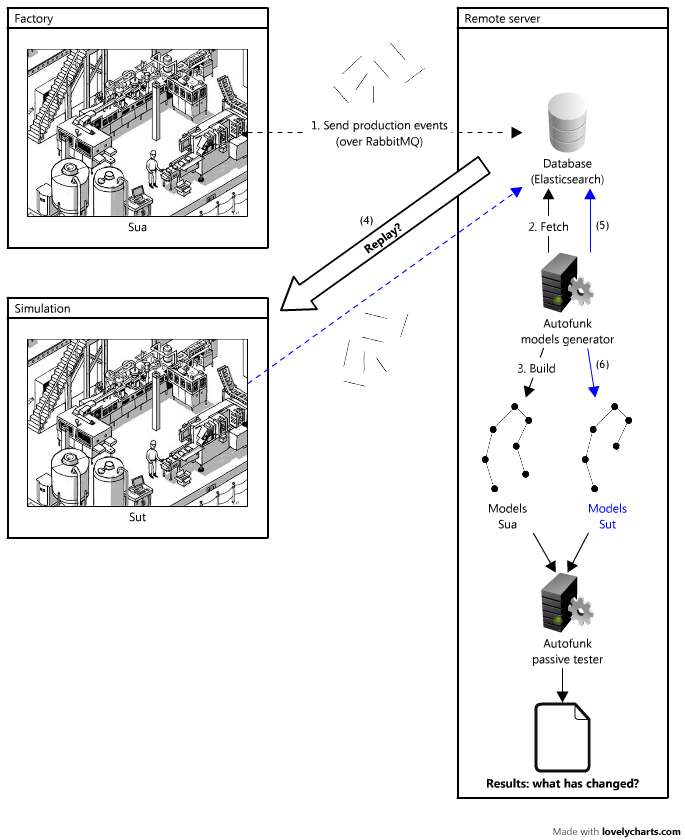
\includegraphics[width=0.96\linewidth]{figures/autofunk_active.png}
    \end{center}

    \caption{Insight of an approach discussed with Michelin to
    use a replay technique with \textit{Autofunk} in order to
    track what has changed between two versions of a production
    system.}
    \label{fig:autofunk_active}
\end{figure}
\clearpage

\subsection{Data mining}
\label{sec:conclusion:testing:data}

Data mining \cite{chakrabarti2006data} is an interdisciplinary
research domain whose goal is to extract information from a data
set. For example, visualization, which we already mentioned in a
previous section, is a component of data mining. In our case,
given the collected trace sets and/or the inferred models, we
have a lot of information available for data mining.

As an example, a side project we quickly set up with Michelin
engineers was to visualize the data collected by
\textit{Autofunk}. We relied on a tool called
\emph{Kibana}\footnote{\url{https://www.elastic.co/products/kibana}}
to show different business metrics, such as the usage rates of
some stores in a workshop, the number of manufactured products
per day, but also the usage rates of the production machines
themselves as depicted in Figure \ref{fig:kibana}. Such
information could be used to create models that might predict
maintenance operations for instance.  The main objective of
\emph{predictive maintenance} \cite{mobley2002introduction} is to
decide when to maintain a system according to its state, which we
could deduce by mining the data contained in the inferred models.

\begin{figure}[h]
    \begin{center}
        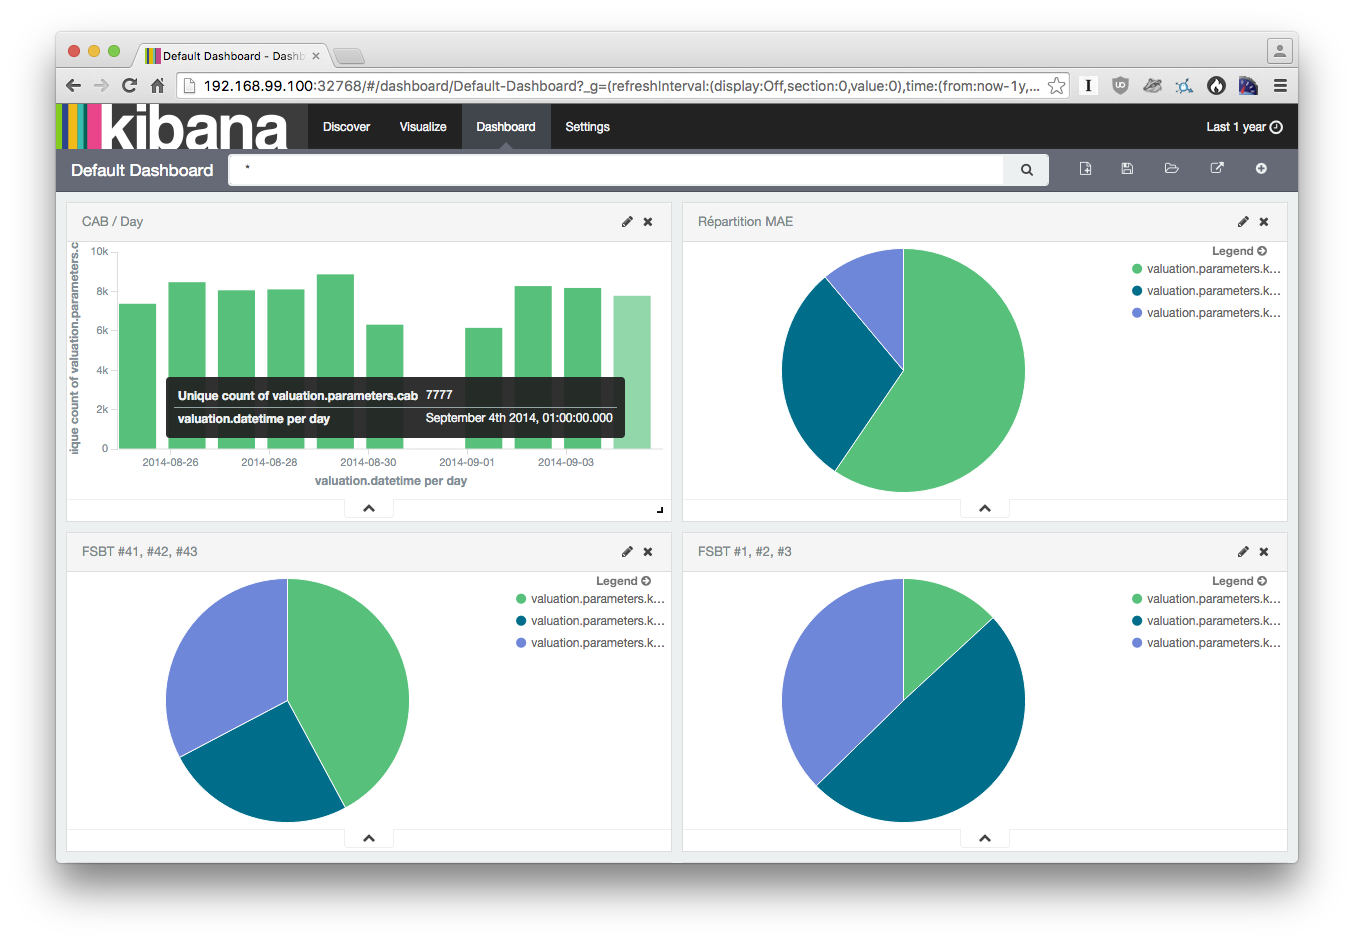
\includegraphics[width=1.0\linewidth]{figures/kibana.png}
    \end{center}

    \caption{Dashboard displaying various business metrics
    created with Kibana, a visualization tool.}
    \label{fig:kibana}
\end{figure}

We could also extract time data from the models. A potential use
case would be to detect slowness in the production lines. That
way, we might highlight imperceptible abnormal functioning
slowing down the whole manufacturing process. This is somehow
related to the \emph{workload-based performance testing} approach
introduced by Avritzer \emph{et al.} \cite{avritzer2002software},
and more generally, to the \emph{Performance Testing}
\cite{vokolos1998performance} and \emph{Knowledge Management}
\cite{pachidi2015performance} fields.

%%%%%%%%%%%%%%%%%%%%%%%%%%%%%%%%%%%%%%%%%%%%%%%%%%%%%%%%%%%%%%%%

\subsection{Refuting our main hypothesis}
\label{sec:conclusion:testing:valid}

As stated in the introduction of this thesis (cf.
\crossref{sec:intro}{sec:intro:problems}), we consider a system
under analysis as a system which behaves correctly. In other
words, such a system does not produce any fault. It is not
entirely unrealistic since this assumption has been validated
with our industrial partner Michelin. In fact, Michelin's
production systems run continuously with only a few scheduled
downtimes, \emph{i.e.} periods when either the whole factory or only a
workshop is unavailable, \emph{e.g.}, for maintenance. Otherwise systems
are fully operational.

That being said, their need for a reliable method to perform
upgrades, which led to the work presented in this thesis,
demonstrates that such systems are not error-proof. Putting it
differently, inferring models representing behaviors of a
software under analysis from production data is compelling, but
it comes at a price: it is likely that \textit{Autofunk} will
infer erroneous behaviors due to a fault that happened in a
production environment, which will not be revealed by our testing
module. It is not an issue when performing, for instance,
robustness testing, but it should not be used for conformance
testing. We were able to perform conformance testing only because
of Michelin's conditions, which we could extend to most of the
existing industrial and manufacturing contexts. Nevertheless, it
cannot be applied in all cases.

Based on this state, we would like to reject such a hypothesis to
perform conformance testing based on our inferred models, but
also to make the models more accurate. We already highlighted a
few paths to improve the accuracy of the inferred models in
Section \ref{sec:conclusion:modelinf:exact}. To go a step
further, we could apply \emph{model checking}
\cite{baier2008principles} if we consider our inferred models as
the system models. Model checking is a verification technique
that explores all possible system states, described in a
\textit{system model}, in a brute-force manner thanks to a model
checker. It is useful to show whether a given system model truly
satisfies a certain property.  Nonetheless, such properties have
to be provided, and we hit a known issue again: the lack of
up-to-date documentation and/or specification of legacy systems.
